\chapter{Google hack}

Dit hoofdstuk gaan we iets grappigs doen waarmee je familie en vrienden kan
foppen. Het einddoel is om het google logo te veranderen naar iets anders
grappigs.

\section{Veranderen van logo}

Als eerste ga naar www.google.be.

\begin{figure}[htpb]
    \centering
    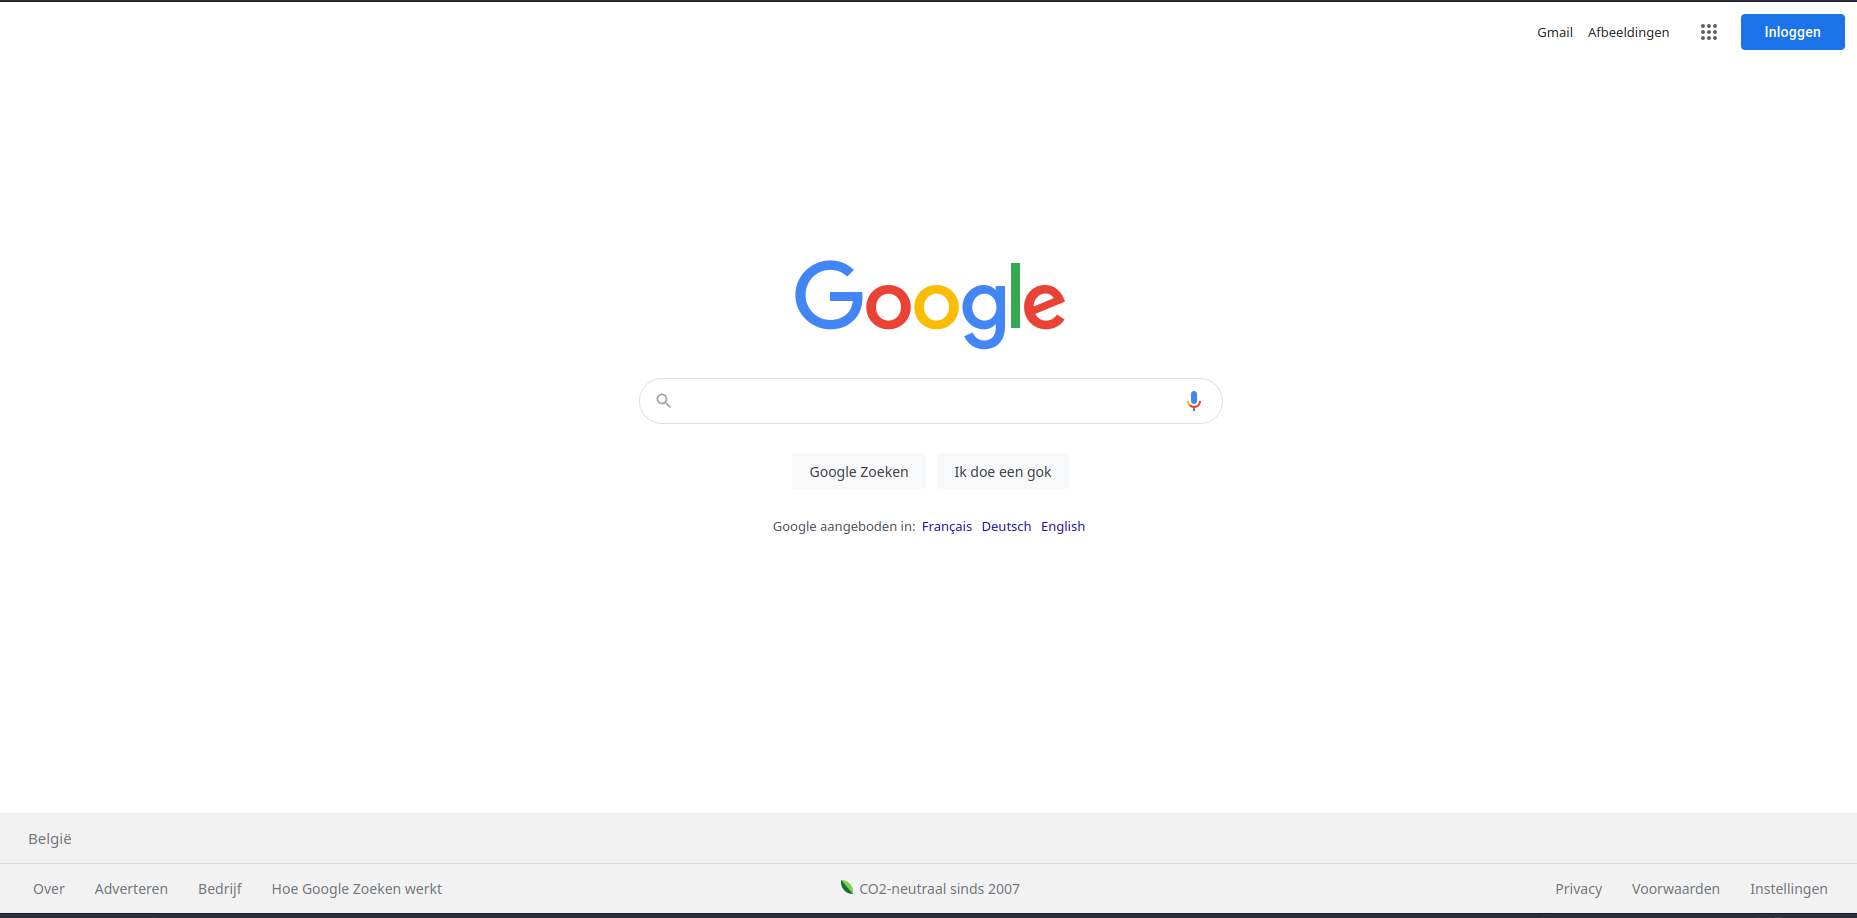
\includegraphics[width=0.6\linewidth]{figures/ga_naar_www_google_be.png}
    \caption{Ga naar www.google.be}
    \label{fig:ga_naar_www_google_be}
\end{figure}

Klik met je rechter muisknop op het \emph{google}-logo en selecteer \emph{inspecteren}.

\begin{figure}[htpb]
    \centering
    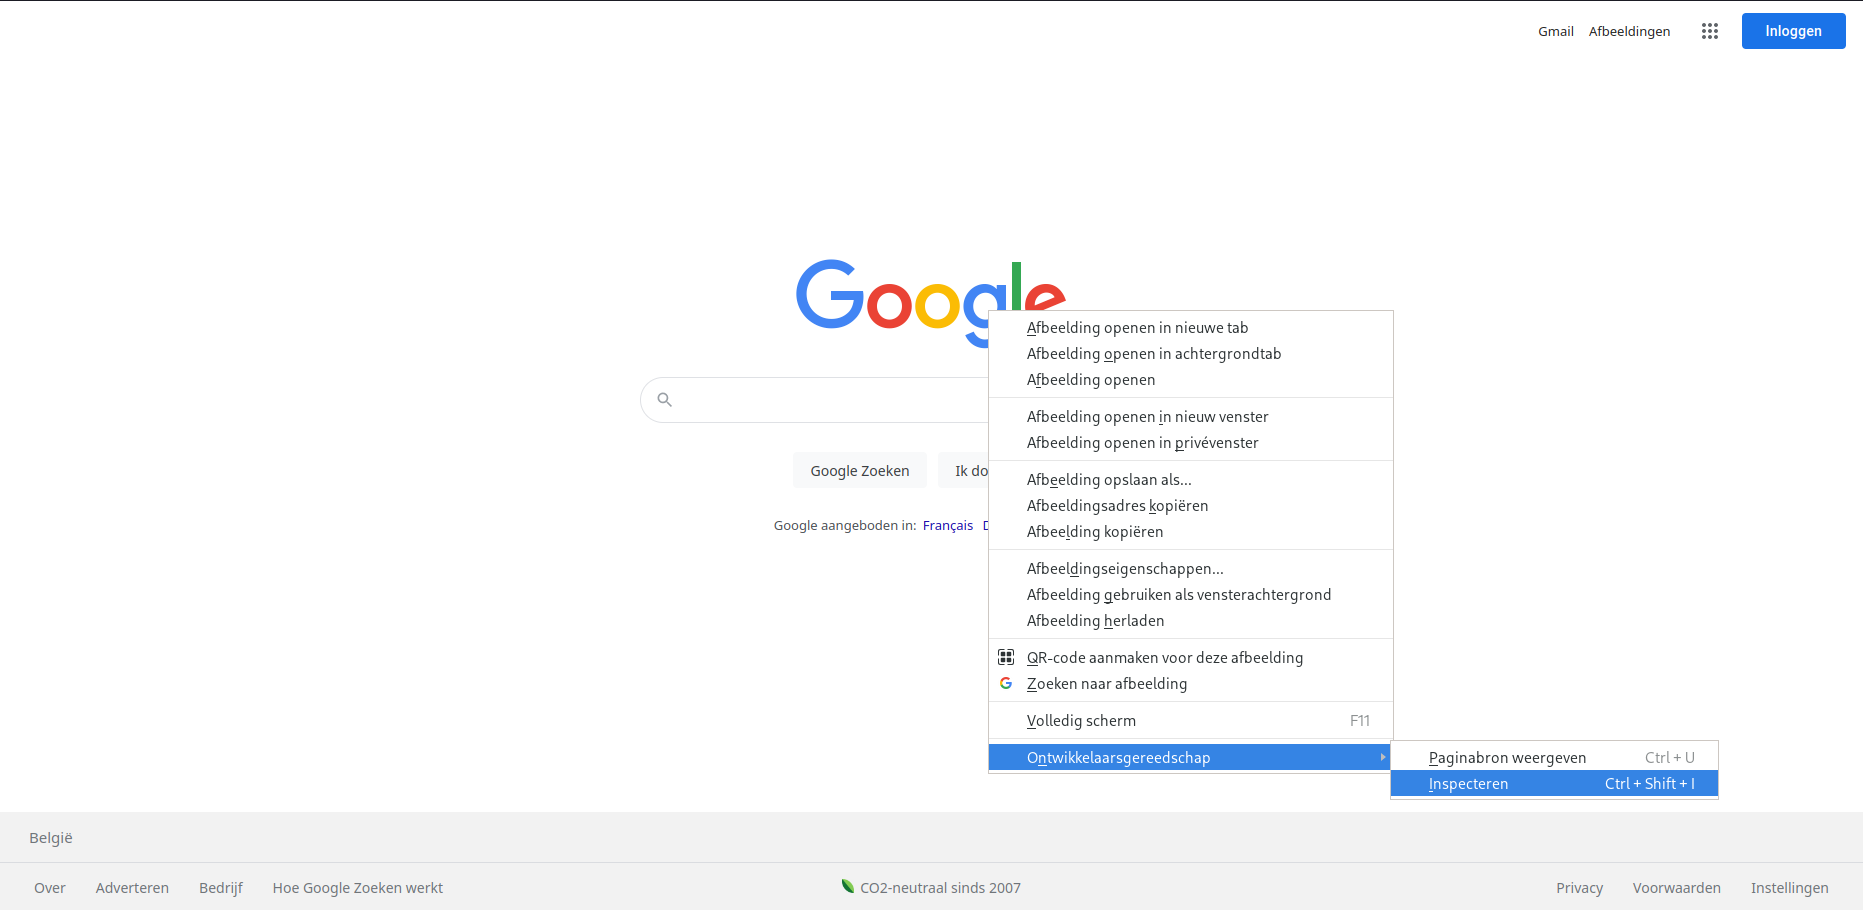
\includegraphics[width=0.6\linewidth]{figures/selecteer_inspecteren_van_google_logo.png}
    \caption{Selecteer inspecteren van Google logo}
    \label{fig:selecteer_inspecteren_van_google_logo}
\end{figure}

We krijgen dan de code te zien voor het \emph{google}-logo. Dit ziet er uit als:
\begin{minted}{html}
<img 
    class="lnXdpd"
    alt="Google"
    height="92"
    src="een zeer lange url.png"
    srcset="een nog langere url.png en dan nog iets"
    width="272"
    data-iml="1662295661263"
    data-atf="1"
    data-frt="0"> 
\end{minted}

Verander dit naar:
\begin{minted}{html}
<img 
    class="lnXdpd"
    alt="Google"
    height="92"
    src="https://www.coderdojobelgium.be/sites/all/themes/coderdojo/images/CoderDojoBelgiumLogo.svg" 
    width="272" 
    data-iml="1662295661263" 
    data-atf="1" 
    data-frt="0">
\end{minted}

We krijgen dan:
\begin{figure}[htpb]
    \centering
    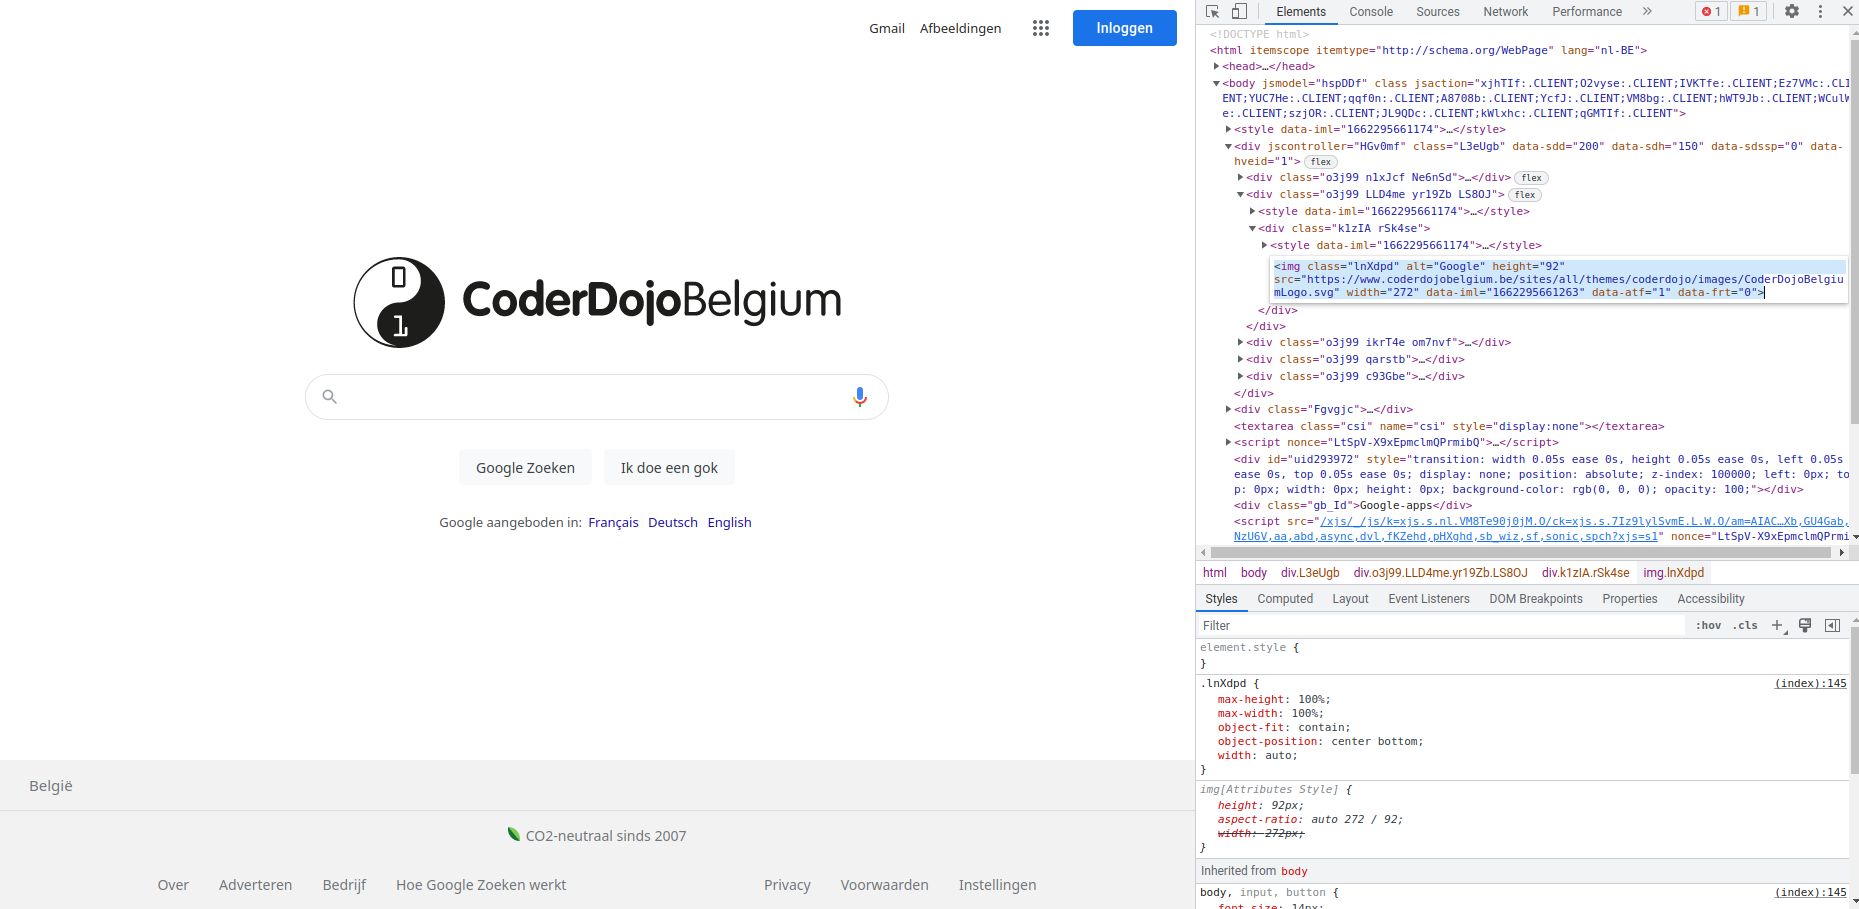
\includegraphics[width=0.6\linewidth]{figures/coderdojo_search.png}
    \caption{Coderdojo search}
    \label{fig:coderdojo_search}
\end{figure}

\section{Veranderen van andere tekst}

Klik op console. Je krijgt dan een manier om direct \emph{JavaScript} te
schrijven. Schrijf nu het volgende en druk dan op \emph{enter}:
\begin{minted}{javascript}
document.designMode = "on"
\end{minted}

\begin{figure}[htpb]
    \centering
    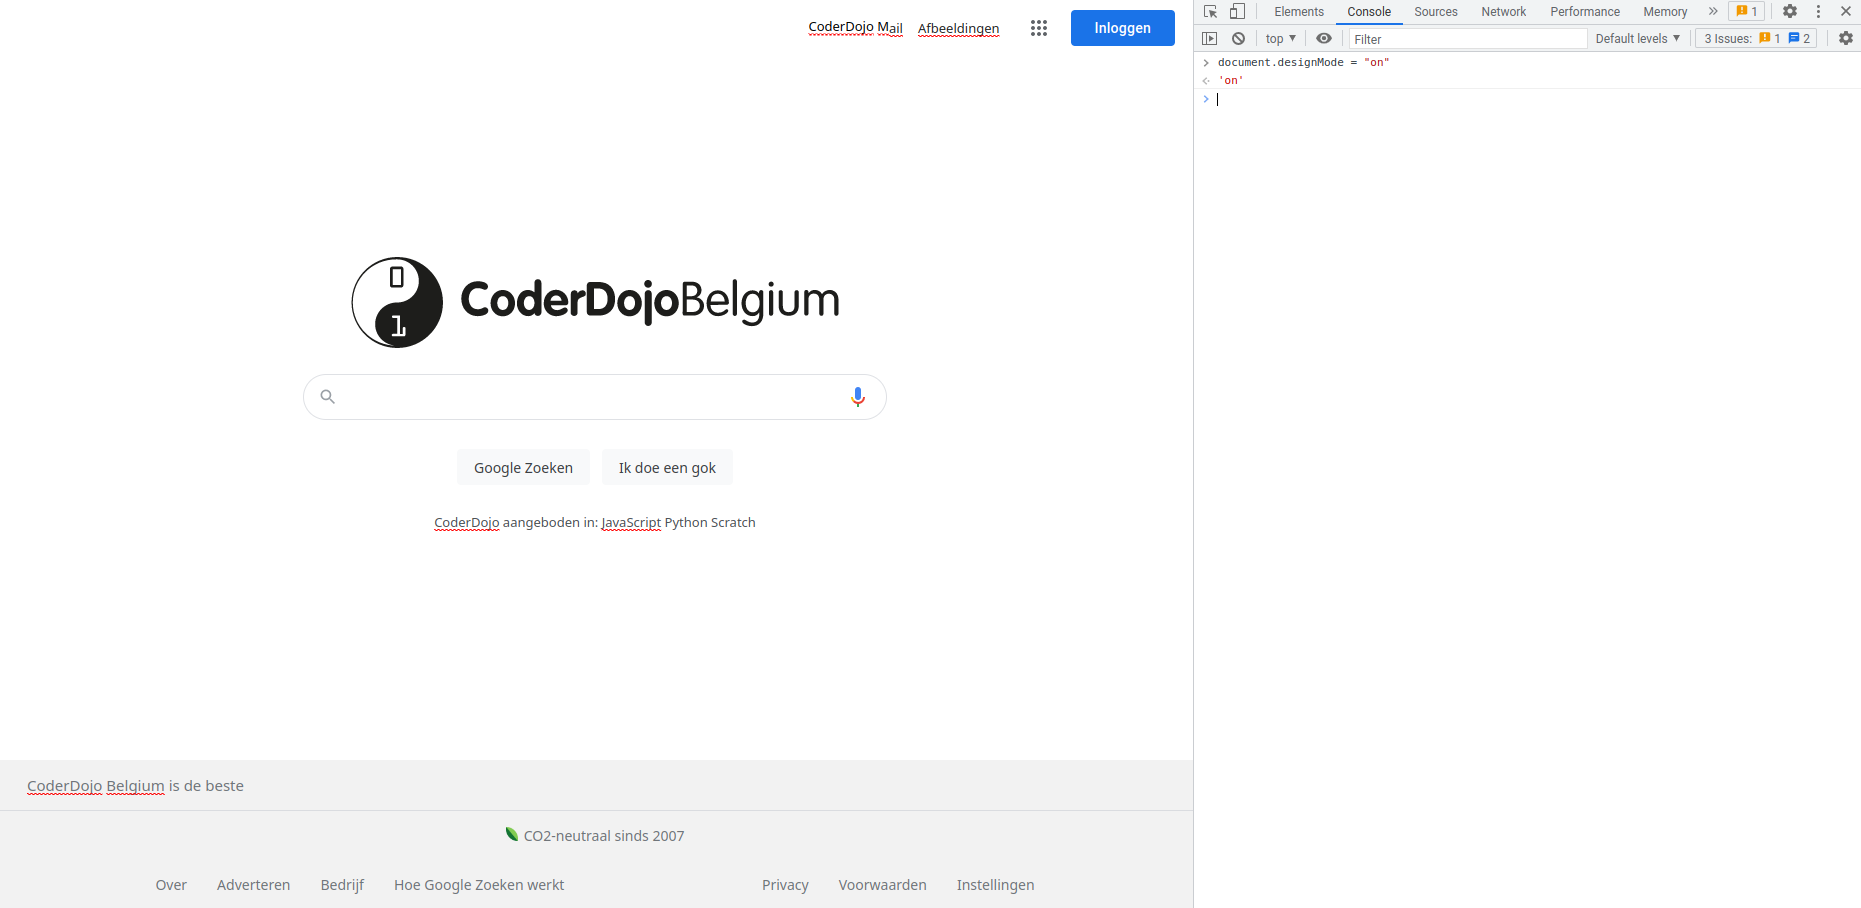
\includegraphics[width=0.6\linewidth]{figures/designer_mode_on.png}
    \caption{Designer mode on}
    \label{fig:designer_mode_on}
\end{figure}

Nu kun je op alle tekst klikken en deze veranderen.
